% This file was converted to LaTeX by Writer2LaTeX ver. 1.0 beta3
% see http://writer2latex.sourceforge.net for more info
% Потом поправлено руками, потому как нагенерилась ересь какая-то.

\documentclass[a5paper]{article}
\usepackage[a5paper, top=17mm, bottom=17mm, left=17mm, right=17mm]{geometry}
\usepackage[utf8]{inputenc}
\usepackage[T2A,T1]{fontenc}
\usepackage[colorlinks,filecolor=blue,citecolor=green,unicode,pdftex]{hyperref}
\usepackage{cmap}
\usepackage[english,russian]{babel}
\usepackage{amsmath}
\usepackage{amssymb,amsfonts,textcomp}
\usepackage{color}
\usepackage{array}
\usepackage{hhline}
\hypersetup{colorlinks=true, linkcolor=blue, citecolor=blue, filecolor=blue, urlcolor=blue, pdftitle=1, pdfauthor=, pdfsubject=, pdfkeywords=}
\usepackage[pdftex]{graphicx}
\usepackage{literat}
\usepackage{indentfirst}

% Text styles
\newcommand\textstyleInternetlink[1]{\textcolor{blue}{#1}}

\sloppy
\pagestyle{empty}

\title{Длинное и пафосное название, содержащее подстроку REAL, как будто кому-то есть до риала дело}

\author{Очень длинный список авторов, гораздо длиннее, чем нужно}
\date{}
\begin{document}

\maketitle
\thispagestyle{empty}

\begin{quote}
\small\noindent
Здесь что-то вроде абстракта.
\end{quote}

\section{Постановка задачи}
Существует большое число систем визуального моделирования, однако
большинство из них обладает довольно существенными, на наш взгляд,
недостатками: практически все известные системы визуального
моделирования ориентированы на однопользовательскую работу с локальным
репозиторием, подавляющее большинство коммерческих реализаций
выпускаются только для определенного семейства операционных систем
(чаще всего – MS Windows), исходные коды таких продуктов недоступны. Те
же, что являются свободно распространяемыми, либо недостаточно зрелы,
имеют довольно ограниченный набор графических редакторов и не имеют
средств для их эффективного создания, либо слабо документированы, либо
уже не поддерживаются.

Отдельно хотелось бы упомянуть CASE-пакет REAL~\cite{real}, разработанный на
кафедре системного программирования математико-механического факультета
СПбГУ. REAL является технологией разработки информационных систем и
систем реального времени и представляет собой набор взаимосвязанных
графических редакторов диаграмм UML 1.4 и SDL-диаграмм, объединенных в
единую среду разработки. Это CASE-средство является открытой системой,
настраемовой под различные задачи (на его основе был создан набор
технологических решений для различных областей, например~\cite{realIt}, и
обладающее способностью интегрироваться с другими средствами
разработки.

Однако, несмотря на богатство функциональных возможностей,
REAL, на наш взгляд, обладал рядом недостатков:

\begin{itemize}
  \item на данный момент со времени выпуска последней версии продукта прошло уже
    более 5 лет, за это время вышла новая версия языка
	UML с расширенным набором диаграмм,
	некоторая реализованная в CASE-пакете
	функциональность стала уже не так актуальна, как раньше;
  \item процесс добавления нового редактора в систему происходил кодированием на
	языке C++ (пусть даже и с учетом факта
	переиспользования компонент), что кажется нам крайне неоптимальным. К
	тому же, добавление нового редактора требовало от разработчиков
	всеобъемлющего знания архитектуры
	CASE-пакета в целом;
  \item изначально реализация графово-графической библиотеки
	CASE-пакета производилась «вручную» на
	основе примитивов, предоставляемых библиотекой
	MFC. В настоящее время такой подход уже
	неприменим: чрезмерно усложняется архитектура продукта, снижается
	производительность, становится невозможным перенос на другие
	платформы.
\end{itemize}

Была предпринята попытка модификации отдельных модулей
REAL (сначала графово-графической библиотеки, а потом и репозитория) с целью устранения указанных
недостатков, однако быстро стало ясно, что осуществление подобного рода
масштабирования и расширения системы неосуществимо, если возможности
для этого не были учтены при изначальном проектировании архитектуры
приложения в целом. 

Таким образом, постановкой задачи нового проекта стало создание подхода
к построению архитектуры и реализация на его основе
CASE-пакета (рабочее название - QReal), обладающего следующими характеристиками:

\begin{itemize}
  \item Распространение под лицензией GPLv2
	(независимость от закрытых, проприетарных библиотек, технологий и
	средств разработки).
  \item Многоплатформенность --– возможность перекомпиляции исходных кодов для
	другой целевой системы без внесения в него изменений.
  \item Распределенность:
  \begin{itemize}
	\item 
	  возможность удаленного доступа к общему репозиторию (как в пределах
	  локальной сети, так и посредством Internet);
	\item возможность конкурентного доступа – наличие системы блокировок (как на
	  уровне диаграмм, так и на уровне элементов) и механизма разграничения
	  прав доступа пользователей.
  \end{itemize}
  \item Наличие средства автоматического создания произвольных графических
	редакторов (в том числе, и пользователями, не владеющими навыками
	программирования).
  \item Набор графических редакторов должен поддерживать, как
	минимум, диаграммы UML 2.1, BPEL и требований.
  \item Внешняя простота архитектуры и прозрачность интерфейсов взаимодействия
	модулей:
  \begin{itemize}
	\item широкие возможности для расширения и масштабирования
	  CASE-пакета;
	\item облегчение процесса его сопровождения.
  \end{itemize}
\end{itemize}

Предполагается, что QReal в дополнение к
графическим редакторам и репозиторию, распространяемым по лицензии
GPLv2, будет включать в себя набор
генераторов форм ввода/вывода, баз данных и исполняемого кода для
различных платформ, распространяемых на коммерческой основе.

\section{Основные концепции создаваемого прототипа}

Поскольку основу коллектива разработчиков
QReal составляют студенты и аспиранты
кафедры системного программирования СПбГУ, было принято базировать
процесс разработки на основе практики прототипирования. Так, на
начальном этапе было создано несколько тестовых демонстрационных
приложений, в результате чего были опробованы принципы и основные
механизмы работы средств, предоставляемых инструментарием Qt, и
сформировано общее представление о будущей архитектуре системы. На
дальнейших этапах архитектура основных компонент пересматривалась,
некоторые из них переписывались практически полностью, однако общие
архитектурные принципы оставались неизменны.

\subsection{Model/View}

После анализа требований к CASE-пакету,
было принято решение строить его архитектуру в соответствии с
парадигмой Model/View.
Шаблон проектирования Model/View (MV) является частным случаем
Model/View/Controller (MVC) и получается из него объединением
\textit{представления} и \textit{контроллера} в одну сущность
(подробнее про MV и MVC можно прочитать в~\cite{somethingAboutMvAndMvc}. Таким образом,
представление становится ответственным и за отображение данных, и за
контроль над действиями пользователя.

Такого рода архитектура, основываясь на тех же принципах, что и
традиционная MVC, дает возможность отделить способ хранения данных от
того, как они представляются пользователю, но предоставляет возможность
создавать более простую инфраструктуру – значительно упрощаются
интерфейсы взаимодействия модулей, снижается интенсивность обмена
служебными сообщениями между ними.

В соответствии с описанной схемой Model/View архитектуру новой
CASE-системы QReal можно представить как комбинацию следующих модулей:

\begin{itemize}
  \item Реализация \textit{Модели}, являющейся надстройкой над
	клиент-серверным репозиторием и реализующей стандартный интерфейс
	взаимодействия компонент в Qt Model/View Framework. В этом смысле сервер репозитория
	является просто хранилищем данных и (при сохранении
	API к клиенту репозитория) может быть при
	необходимости заменен практически без изменения остальных компонент
	системы (включая саму реализацию модели).
  \item 
	Набор редакторов и элементов графического интерфейса пользователя,
	являющихся реализациями представлений.
\end{itemize}

Следует заметить, что если бы подобная архитектура строилась нами в
соответствии с парадигмой Model/View/Controller,
функциональность контроллера брала бы на себя логика графических
редакторов, а реализациями представления были бы только рабочие области
этих редакторов.

Подобное разнесение реализации одной сущности (графического редактора)
по разным программным модулям, во-первых, снижает логическую
целостность архитектуры, препятствует полноценной инкапсуляции в
редакторе его функциональности, а во-вторых, требует создания
дополнительных компонент и их внешних интерфейсов, что в свою очередь,
как правило, увеличивает поток служебных сообщений между компонентами и
вполне может сказаться на производительности всего
CASE-пакета.

\subsection{Графический интерфейс. Выбор инструментария}

Графический интерфейс CASE-пакета обычно
содержит вполне определенный набор элементов. В
QReal они представлены следующими
компонентами (см. рис. 1):

\begin{itemize}
  \item \textit{Инспектор объектов (Object Explorer).} Представляет
	собой дерево объектов, содержащее все элементы в открытом в данный
	момент репозитории, отсортированные по их типам. Необходим для
	обозревания всего проекта в целом. Также инспектор объектов бывает
	удобен, например, при добавлении на текущую диаграмму уже существующего
	в проекте объекта (например, не принадлежащего никаким диаграммам). В
	таком случае необходимый элемент может быть добавлен на диаграмму
	"перетаскиванием" в ее рабочую область, посредством соответствующего
	пункта контекстного меню или другими способами.
  \item \textit{Инспектор диаграмм (Diagram Explorer).} Отображает все
	созданные в рамках данного проекта пользовательские диаграммы и
	элементы на них в виде дерева. Один и тот же элемент в общем случае
	может принадлежать неограниченному числу диаграмм, тогда визуально в
	инспекторе он будет отображаться как потомок всех диаграмм, которым он
	принадлежит (в инспекторе объектов, разумеется, всем этим «копиям»
	будет соответствовать один элемент). Также инспектор может
	использоваться для переключения диаграмм, отображаемых в рабочей
	области редактора.
  \item \textit{Редактор свойств (Property Editor).} При выделении
    элемента, предоставляет информацию о нем и позволяет изменять значения
	его атрибутов.
  \item \textit{Палитра компонентов.} Отображает все возможные для добавления на
	диаграмму визуальные элементы. 
  \item \textit{Меню.} Содержат основные операции над репозиторием
	(прервать/осуществить соединение с сервером репозитория), диаграммами
	(создать/удалить диаграмму, сменить диаграмму, отображающуюся в рабочей
	области редактора, распечатать текущую диаграмму, отменить/повторить
	последнее действие и т.п.), объектами (например, удалить объект с
	диаграммы/из репозитория) и другие.
  \item \textit{Панели инструментов (Toolbars)}. Содержат
	ярлыки наиболее важных или часто используемых операций меню или
	действий пользователя.
  \item \textit{Рабочая область графического редактора диаграмм}. Основная
	рабочая область CASE-пакета. С ее помощью
	осуществляется отображение и модификация создаваемых пользователем
	диаграмм. Редактор содержит в себе полную информацию о содержащихся
	элементах на диаграммах выбранного типа и логические правила их
	интерпретации.
\end{itemize}


\begin{figure} [ht]
  \begin{center}
    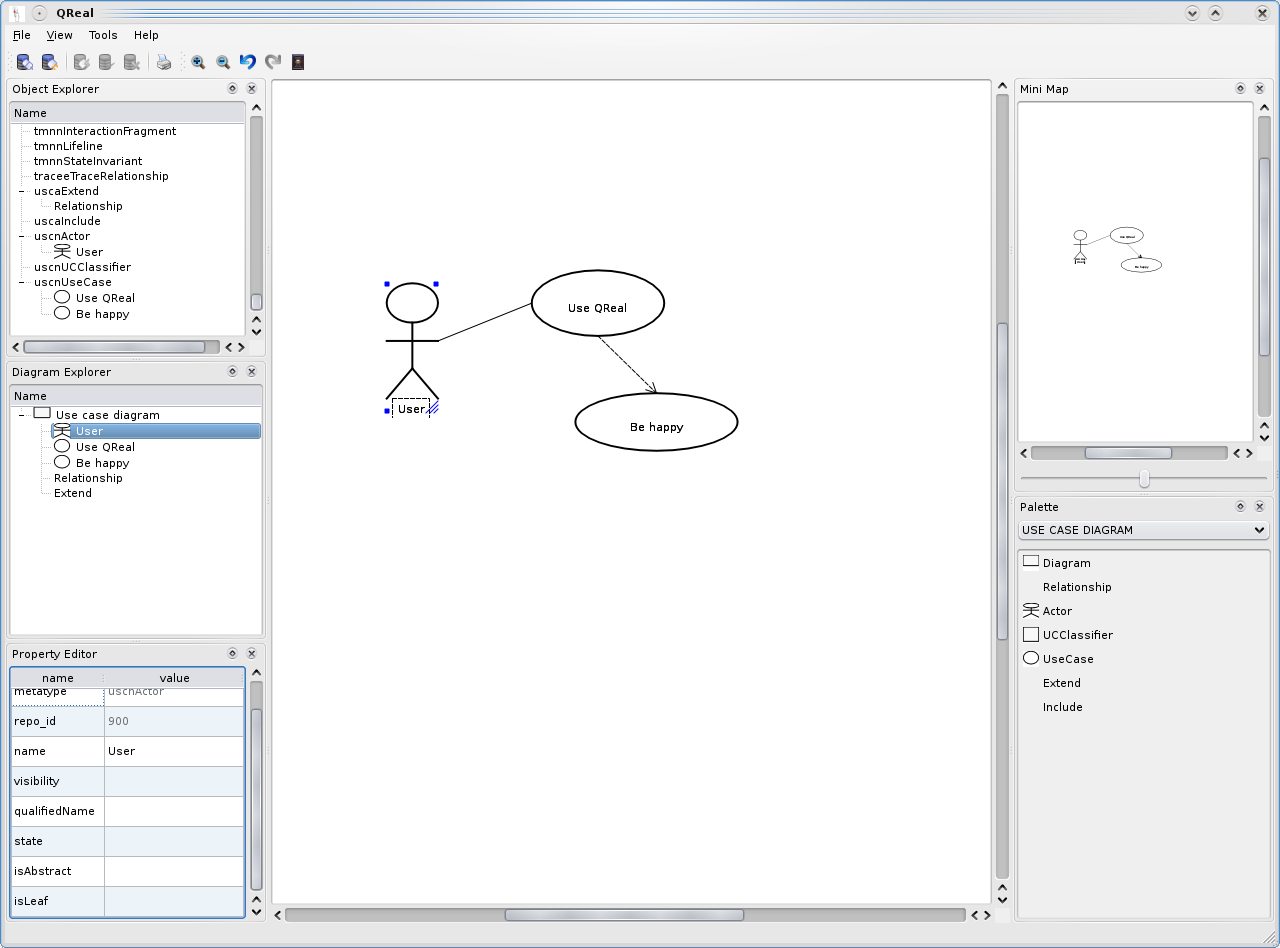
\includegraphics[width=14.704cm,height=10.918cm]{draft04-img1.png}
    \caption{Главное окно QReal}
    \label{mainWindow}
  \end{center}
\end{figure}

% {\centering 
% 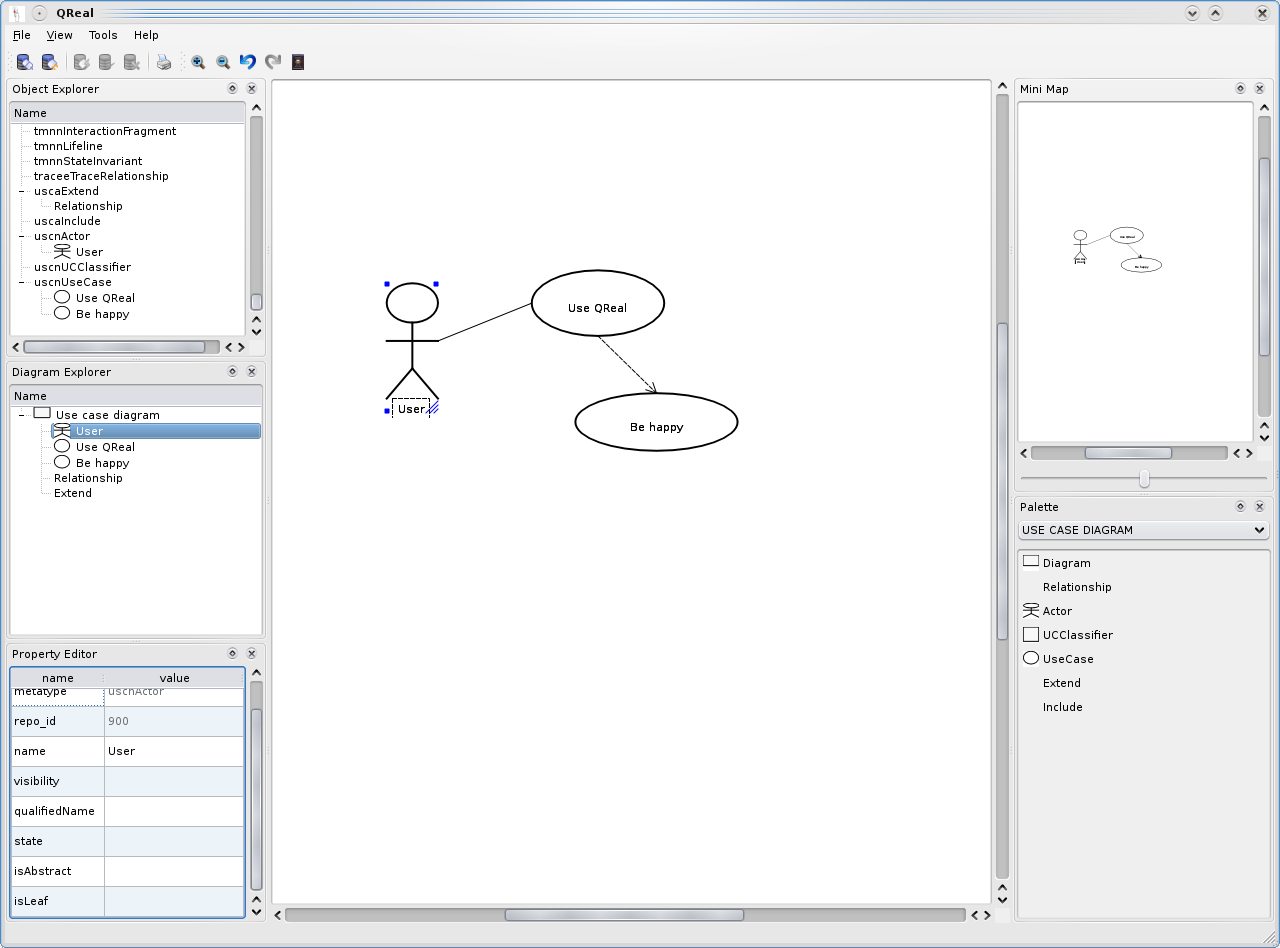
\includegraphics[width=14.704cm,height=10.918cm]{draft04-img1.png}
% \par}
% {\centering\selectlanguage{russian}
% Рис. 1. Главное окно QReal}
% \par}

Следует заметить, что реализация подобного рода элементов графического
интерфейса в общем случае является платформо-зависимой задачей, т.е.
требует использования системных графических библиотек, что противоречит
предъявляемому нами к разрабатываемому CASE-пакету требованию
многоплатформенности. Известно несколько способов решения задач такого
рода:

\begin{itemize}
  \item Использование переносимости на уровне бинарного кода. В этой области
	наиболее распространено использование Java в
	качестве языка разработки. Программы на Java могут быть транслированы в
	байт-код, выполняемый на виртуальной Java-машине. Т.к. байт-код полностью не
	зависит от целевой операционной системы, Java-приложения могут работать
	на любом устройстве, для которой существует реализация виртуальной машины. 
  \item Переносимость приложения на уровне исходных кодов. Это достигается путем
	использования многоплатформенных инструментариев
	(toolkits), являющихся надстройками над
	системными библиотеками и инкапсулирующих в себе реализацию базовых
	графических примитивов для различных операционных систем. Библиотеки
	подобного рода предоставляют единый интерфейс для работы с ними вне
	зависимости от используемой операционной системы, что позволяет
	добиться переносимости создаваемого приложения на уровне исходных
	кодов. Наиболее распространенными готовыми решениями в данной области
	являются инструментальные средства Qt и	GTK+.
\end{itemize}

В процессе разработки архитектуры и реализации прототипов основных
модулей требуемого CASE-пакета было решено
ориентироваться на возможности инструментария
Qt. Этот выбор показался нам тогда удачным
по следующим причинам:

\begin{itemize}
  \item Qt казался динамически развивающимся
	проектом: за те полгода, когда формировалась идея о написании новой
	CASE-системы и закладывались основные
	требования к ней, было выпущено 2 новых версии этого инструментария,
	каждая из которых существенно расширяла функциональные возможности
	предыдущей.
  \item 
	Начиная с версии 4.0 (на начало работ по созданию прототипа текущей была
	версия 4.1), Qt уже не позиционируется
	разработчиками как набор графических библиотек. Это полноценный
	инструментарий для разработки многоплатформенных приложений –-- со
	временем в в его состав вошли все основные классы, которые могут
	потребоваться при разработке программного обеспечения любой сложности:
	начиная от элементов графического интерфейса и заканчивая классами для
	работы с сетью, базами данных или XML.
  \item Начиная с Qt версии 4 в его состав входит Qt Model/View
	Framework, который предлагает удобные
	средства для создания приложений в соответствии с парадигмой
	Model/View и предоставляет для использования набор готовых реализаций стандартных
	моделей и представлений.
  \item Основные члены команды разработчиков уже имели опыт разработки
	приложений с использованием этого инструментального средства.
\end{itemize}

К возможным недостаткам выбранного способа решения задачи достижения
многоплатформенности создаваемого CASE-пакета некоторые могли бы отнести
необходимость перекомпиляции исходных кодов при переносе на другую
платформу. Этот довод кажется нам неубедительным, т.к. перекомпиляция
CASE-пакета (требуемая прежде всего при переходе на другую операционную систему или платформу) конечным
пользователем предполагается осуществляемой крайне редко, т.е.
отношение времени компиляции исходных кодов к общему времени работы с
продуктом крайне невелико.

В итоге оказалось, что данный выбор был весьма удачным, ибо на текущий
момент инструментарий развился до версии 4.5, предлагая разработчикам
помимо всего прочего инструменты для работы со звуком (начиная с
Qt 4.4), возможности для эффективного использования модуля Webkit для интеграции
приложений с World Wide Web (начиная с Qt 4.5) и даже удобную среду для
разработки приложений Qt Creator. Кроме того, начиная с версии 4.5,
пакет Qt распространяется в соответствии с лицензией LGPL, что дает возможность для
использования его в коммерческих приложениях.

\subsection{Репозиторий на основе реляционной СУБД}

Репозиторий является ответственным за хранение данных и предоставление
интерфейсов доступа к ним для других компонент. В связи с требованием
распределенности, предъявляемым к разрабатываемому
CASE-пакету (а именно, возможности удаленного доступа пользователей к репозиторию), было принято решение
реализовывать репозиторий в соответствии с архитектурой клиент/сервер.
Таким образом, клиентская часть репозитория будет встраиваться в сам
CASE-пакет, а серверная может быть физически размещена на другом компьютере, доступном по локальной сети
или через интернет. Серверная составляющая может быть реализована:

\begin{itemize}
  \item на основе стандартных средств версионного контроля (например,
	CVS, Visual SourceSafe или Subversion);
  \item в виде хранилища данных с помощью набора плоских файлов;
  \item как надстройка над реляционной СУБД (большого опыта работы с
	объектно-ориентированными СУБД участники проекта в то время не имели).
\end{itemize}

Последний вариант показался нам на тот момент наиболее удачным по
следующим причинам:

\begin{itemize}
  \item системы управления базами данных по своему назначению ориентированы на
	хранение и эффективную обработку больших объемов информации, поэтому с
	ростом числа пользовательских диаграмм и элементов на них потери в
	производительности репозитория окажутся незначительными;
  \item наличие механизмов блокировок (на уровне таблиц и записей), транзакций и
	разграничений прав пользователей дает возможность для организации
	многопользовательского конкурентного доступа к репозиторию практически
	«из коробки»;
  \item использование простейших утилит администрирования, поставляющихся в
	составе СУБД, позволяет осуществлять импорт/экспорт содержимого базы
	данных в виде ее снимков (snapshots). При
	этом данные сериализуются в виде скриптов на языке запросов
	SQL (точнее, его подмножестве DDL) и могут использоваться для помещения в
	систему контроля версий, внутреннего резервного копирования, быстрого
	переноса на другую СУБД или других служебных целей;
  \item возможность физического разнесения клиента и сервера репозитория, а
	также унифицированные средства для работы с разными СУБД,
	представляемые Qt, снимают
	ограничения на выбор как используемой СУБД, так и операционной системы
	серверной части, поэтому CASE-пакет
	становится более гибким в настройке и использовании;
  \item поддержка системами управления базами данных стандартных сетевых
	протоколов TCP/IP снимает необходимость реализации сетевых компонент серверной части и
	позволяет организовать доступ к серверу репозитория из глобальных
	сетей, в том числе и из Интернет;
  \item в условиях сжатых сроков создания прототипа
	CASE-системы казалось разумным использовать уже готовые отлаженные технологии и средства 
	--– времени на "изобретение велосипеда" или исследование сторонних или
	экспериментальных решений просто не было.
\end{itemize}

Хранимые данные (информация о диаграммах и элементах) в общем виде имеют
графовое представление, к тому же один элемент может принадлежать
разным диаграммам, поэтому для их хранения с использованием реляционных
таблиц базы данных применялось их специальное преобразование. Для
хранения данных использовалось несколько таблиц:

\begin{itemize}
  \item metatable --– информация о поддерживаемых типах элементов;
  \item nametable --– список существующих в репозитории
	элементов вместе с их идентификаторами, типами и набором свойств, общих
	для всех элементов (например, имени);
  \item diagram --– данные о потомках объектов (в
	частности, о содержимом всех диаграмм и контейнеров). Получение списка
	дочерних элементов является очень частой задачей, для ускорения чего и
	была введена эта таблица. Также в этой таблице хранится конфигурация
	элемента в рамках каждого "родителя" (координаты, размеры элементов,
	точки перелома ассоциаций и т.п.);
\end{itemize}

Примеры SQL-запросов к такого вида таблицам
и более подробное описание схемы базы данных можно найти в дипломной
работе Г. Никандрова~\cite{nikandrov}.

\subsection{Генеративный подход к созданию редакторов}

CASE-пакет по определению –-- это система
визуального моделирования, в состав которой входит определенное число
графических редакторов. И будь то редакторы бизнес-процессов, схем баз
данных, компонент программного обеспечения или структуры организаций,
по своему внутреннему устройству они будут довольно похожи. Так,
редактор инкапсулирует в себе информацию о наборе объектов, допустимых
на диаграммах данного типа, должен быть способен правильно
интерпретировать хранящиеся в репозитории значения атрибутов элементов
(например, использовать некоторые из них как параметры при их
отрисовке) и иметь представление о логических правилах размещения
элементов на соответствующих типах диаграмм (например, возможность
соединять некоторые элементы ассоциациями, возможность одних элементов
быть контейнером для других и т.д.).

Создавать набор таких редакторов кодированием их "вручную" кажется нам
неразумным по следующим причинам:

\begin{itemize}
  \item с ростом числа редакторов значительно снижается сопровождаемость кода;
  \item слабая расширяемость --– добавление новой функциональности требует
	изучения (а нередко и существенного рефакторинга) уже существующего
	кода;
  \item опасная масштабируемость --– создание дополнительного редактора,
	являющегося типовым для данного CASE-средства, чаще всего будет
	осуществляться методом Copy/Paste с
	дальнейшими доработками полученного после копирования, что влечет как к
	появлению дополнительных ошибок, связанных с неполнотой вносимых
	правок, так и к размножению уже существующих;
  \item происходит неизбежное усложнение внутреннего устройства модуля
	редакторов, и, как следствие, усложнение и громоздкость архитектуры
	CASE-пакета в целом.
\end{itemize}

В соответствии с этим был предложен следующий подход к автоматическому
созданию графических редакторов: 

\begin{itemize}
  \item путем анализа типовых редакторов выделяется базовая функциональность
	абстрактного редактора, которая кодируется "вручную" на целевом языке
	высокого уровня (в нашем случае, на C++);
  \item в соответствии с проведенным анализом, специфика метамоделей нужных
	диаграмм (или наиболее полное их подмножество) исчерпывающим образом
	описывается с помощью специального XML-формата;
  \item по этим описаниям генерируется C++ код,
	который в совокупности с базовой функциональностью полностью реализует
	требуемую функциональность описанных диаграмм.
\end{itemize}

Для того, чтобы создание такого набора редакторов и интеграция его в
CASE-пакет стало возможным, в нем была реализована следующая инфраструктура:

\begin{itemize}
  \item "ядро", обеспечивающее функциональность абстрактного редактора:
    \begin{itemize}
      \item способность элементов принадлежать диаграммам (в том числе, способность
	    одного элемента принадлежать неограниченному числу диаграмм);
	  \item способность получать значения нужных атрибутов из репозитория и
	    отслеживать изменения его содержимого;
	  \item способность элементов отрисовываться в пределах рабочей области
	    диаграммы;
	  \item способность ассоциаций соединять элементы и способность элементов
	    присоединять к себе ассоциации;
	  \item способность (абстрактного) элемента быть контейнером для других;
	  \item способность элемента реагировать на действия пользователя (например, на
	    выделение курсором мыши, перемещение, изменение размеров) и т.п.
    \end{itemize}
  \item наследуемые от «ядра» классы, определяющие специфику конкретных типов
	диаграмм:
	\begin{itemize}
	  \item набор допустимых для каждого конкретного типа диаграмм элементов;
	  \item их графическое представление и параметризация его значениями атрибутов
		этих элементов;
	  \item стиль начертания ассоциаций, форма и тип возможных стрелок;
	  \item логические правила, специфичные для данного типа диаграмм (например,
		правила соединения элементов ассоциациями) и т.п.
	\end{itemize}
\end{itemize}

Необходимый для описания метамоделей диаграмм формат должен обладать
следующими возможностями:

\begin{itemize}
  \item задание графического представления элемента в текстовом виде (для
	элементов) или способа начертания линий и задания формы с типа стрелок
	(для ассоциаций);
  \item задание параметризации статического изображения элемента содержимым
	репозитория (например, отображение имени элемента);
  \item описание набора атрибутов элементов: поддержка как основных типов данных
	(строки, числа, логический тип, перечисление), так и возможность
	создания пользовательских;
  \item указание факта наследования элементов;
  \item описание логики ассоциаций: задание для каждого конца ассоциации набора
	допустимых для соединения с ним элементов, задание атрибутов ассоциаций
	(например, множественности или метки) и т.п.
\end{itemize}

Формат должен основываться на XML и иметь
простую структуру. Тогда создание новых редакторов или внесение
изменений в уже существующие не требует ни навыков программирования, ни
знания внутреннего устройства всего CASE-пакета и может осуществляться
пользователями напрямую.

В ходе работ над реализацией прототипа CASE-пакета формат, обладающий описанными
характеристиками, был разработан А.Симоновой и подробно описывается в
ее дипломной работе~\cite{simonova}.

\subsection{Реализация представлений}

В соответствии с предлагаемой инфраструктурой для интеграции редакторов
в CASE-пакет была создана следующая иерархия классов:

% TODO: разобраться, как привести в божеский вид. Пока решил не трогать.
{\centering [Warning: Draw object ignored][Warning: Draw object ignored]
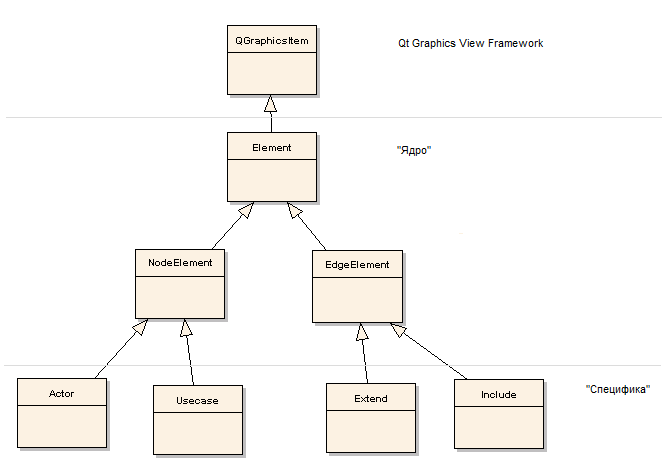
\includegraphics[width=10.786cm,height=9.038cm]{draft04-img2.png} \par}

\begin{figure}
\begin{center}
\begin{minipage}{2.849cm}

«Ядро»
\end{minipage}
\end{center}
\end{figure}
\begin{figure}
\begin{center}
\begin{minipage}{6.024cm}
{\selectlanguage{english}
Qt Graphics View Framework}
\end{minipage}
\end{center}
\end{figure}
\begin{figure}
\begin{center}
\begin{minipage}{3.801cm}

«Специфика»
\end{minipage}
\end{center}
\end{figure}
\subparagraph[Рис. 2. Иерархия классов элементов графических
редакторов]{Рис. 2. Иерархия классов элементов графических редакторов}


Класс QGraphicsItem является базовым классом всех графических элементов Qt
Graphics View Framework. На его основе строятся все
стандартные классы графических элементов Qt
и могут определяться пользовательские. Путем обработки возникающих
событий он берет на себя решение задач по определению геометрии
элемента (например, поворота или масштабирования), параметров его
отрисовки (видимость, возможность перехвата событий выделения,
перемещения элемента пользователем и т.п.), выявлению коллизий
(обработка пересечений и уровней наложений) и способах взаимодействия
элементов (композиции объектов, возможность одних быть контейнером для
других и т.п.).

Класс Element осуществляет базовую связь
между элементом логической модели в репозитории и объектом
\textit{представлений}, осуществляющим его отображение. Основной
функциональностью данного класса является получение и хранение
"указателя" (индекса) на элемент логической модели репозитории,
визуализацией которого является элемент, наследующийся от этого класса.

Классы NodeElement и EdgeElement реализуют основные сущности,
присутствующие на абстрактной диаграмме –-- вершину и ребро/дугу графа. А
так как в основе логической модели любой диаграммы (за некоторыми
исключениями, которые можно обрабатывать особо) лежит граф, все
элементы, которые потенциально могут присутствовать на диаграмме,
являются потомками одного из этих классов.

Так, экземпляры класса NodeElement и (что для
нас гораздо важнее) его потомков обладают следующей функциональностью:

\begin{itemize}
  \item способность иметь порты для присоединения к ним ассоциаций. Порт может
	быть либо точкой, либо отрезком (в таком случае, каждая точка отрезка
	считается портом);
  \item хранение информации о той части логической модели, в которую входит
	данный элемент (например, ссылки на присоединенные к нему ассоциации,
	число и список дочерних элементов в случае, если элемент является
	контейнером и т.п.);
  \item наличие обработчиков изменений размера элемента и его перемещения
	пользователем, синхронизация этих действий с логически связанными с ним
	объектами (например, адекватное изменение положения присоединенных к
	элементу ассоциаций при перемещении его в пределах рабочей области);
  \item сохранение и загрузка данных о своем расположении (размер, координаты)
	на диаграмме из репозитория;
\end{itemize}

Экземпляры класса EdgeElement и его потомков, в свою очередь, обладают следующей функциональностью:

\begin{itemize}
  \item способность присоединять свои концы к портам элементов. В нашей
	реализации все ассоциации являются бинарными, каждая ассоциация имеет 2
	конца (для направленных ассоциаций выделяется их начало и конец);
  \item способность ассоциаций иметь надпись (метку) над ней;
  \item возможность задания ассоциации ломаной линией;
  \item способность хранения информации о своем расположении и присоединенных
	элементах в репозитории.
\end{itemize}

\subsection{Генерация специфики диаграмм}

Как уже говорилось ранее, классы Element, NodeElement и
EdgeElement не предназначены для создания их объектов, а служат лишь для задания набора базовых операций над
элементами и ассоциациями абстрактного типового редактора. В
соответствии с предложенным подходом создания редакторов, вся специфика
элементов конкретных диаграмм формализуется с помощью специального
XML-формата.

Созданные описания метамоделей подаются на вход специальной
утилите-генератору, которая осуществляет анализ предоставленных ей
XML-документов, в результате чего для
каждой сущности (как для элемента, так и для ассоциации) определяется:

\begin{itemize}
  \item уникальный в рамках всех метамоделей идентификатор типа. В дальнейшем
	используется для именования файлов графических описаний, формирования
	имени типа и в некоторых других операциях;
  \item имя типа (название сущности на естественном языке). Используется для
	именования соответствующих элементов палитры компонентов и инспектора
	объектов;
  \item список свойств сущности с указанием их типа. Поддерживаются основные
	типы данных (число, строка, текст, логический тип, перечисление и
	некоторые другие), также допускается задавать в качестве типа свойства
	ссылку на другую сущность;
  \item список родительских элементов. Сущность наследует свойства и логику
	родительских элементов, не перекрываемые ее собственными.
\end{itemize}

Дополнительно, сущности, которые описаны как
Node (т.е. элементы), имеют секцию описания
их графического представления, в которой чаще всего находится
соответствующее описание графического представления элемента (в первых
версиях использовался язык SVG). Это
описание сохраняется в виде файла на диске и будет использоваться в
дальнейшем в процессе работы CASE-пакета
как для отрисовки элементов данного типа в рабочей области редактора
диаграмм, так и для создания иконок для палитры компонентов, инспектора
объектов и диаграмм. Изображения, описанные на языке SVG, являются статичными, поэтому для их
параметризации содержимым репозитория (значением соответствующих
свойств элемента) используется специальная
XML-секция. Важной особенностью предлагаемого подхода к параметризации
SVG-изображений является то, что используются расширенные соответствующим образом теги
HTML. Такой выбор не случаен –-- используемый
для отображения получаемых строк класс QTextDocument обладает способностью
интерпретировать основные теги HTML
(поддерживаемое подмножество тегов можно посмотреть в~\cite{htmlInQt}, что дает
богатые возможности для форматирования подставляемых из репозитория
значений. В ходе разбора соответствующих секций XML-описаний генератор заменяет теги
параметризации соответствующим C++ кодом для
получения нужных значений атрибутов элемента. При этом теги
форматирования текста сохраняются. Во время выполнения получаемого
таким способом такого кода произойдет обращение к репозиторию,
получаемое значение атрибута будет получено, отображено в рабочей
области редактора (поверх статичного SVG-изображения элемента), и требуемая
параметризация будет осуществлена.

Также при описании элементов возможно задание портов --– областей его
графического отображения, к которым возможно присоединение ассоциаций.
Формат (а, следовательно, и генератор) поддерживает задание портов двух
типов --– точка и отрезок (в случае последнего ассоциация может быть
прикреплена к любой точке отрезка). Вся функциональность по обработке
присоединения к портам и адекватного отображения ассоциаций при
изменении размера/движении элемента реализована в классах
NodeElement и EdgeElement, в генерируемых классах
конкретных элементов достаточно лишь указать тип и расположение порта.

Для сущностей, описанных как Edge (т.е. для
ассоциаций), для каждого из концов ассоциации указывается набор типов
элементов, к которым она может быть прикреплена. Также существует
возможность указать тип начертания линии ассоциации при ее визуальном
отображении. Типы линий, допустимые в описаниях, являются аналогами
соответствующих значений перечисления Qt::PenStyle, что
во-первых, дает богатые возможности для выбора стиля начертания линий
(сплошная, прерывистая, точечная, точка-тире, точка-точка-тире), а
во-вторых сводит к минимуму кодирование поддержки соответствующей
функциональности.

Также при описании ассоциаций возможно задание формы и стиля закраски
стрелок. Так, формат поддерживает задание обычных стрелок и стрелок в
виде ромба (как закрашенные, так и нет для обоих вариантов).
Способность ассоциации корректно отрисовывать на своих концах стрелки
нужной формы реализована в классе EdgeElement, в генерируемых классах
необходимо лишь задать ее конкретную форму и стиль заливки.

После фазы разбора XML-описаний
метамоделей, генератор переходит в фазу анализа полученной информации.
Для каждой сущности осуществляется построение полного набора ее свойств
(с учетом возможности наследования элементов), для каждой ассоциации –--
полный список возможных для присоединения элементов (для каждого из
концов), проверяется ссылочная целостность. В случае, если определенный
элемент ссылается на несуществующий элемент, выдается предупреждение и
некорректная ссылка удаляется. 

В ходе заключительной фазы происходит генерация необходимых артефактов.
А именно, создаются:

\begin{itemize}
  \item классы на языке C++ всех элементов и
	ассоциаций диаграмм. Они наследуются от базовых классов
	NodeElement и EdgeElement и определяют специфику
	задаваемых сущностей --– для элементов задается файл с
	SVG-описанием его графического
	представления, устанавливаются размеры отображаемого изображения,
	указываются число, тип и расположение портов элемента, задается
	параметризация изображения значениями атрибутов элемента хранящихся в
	репозитории; для ассоциаций задается стиль начертания их линий, форму и
	стиль заливки стрелок (если они есть);
  \item файлы с SVG-описаниями графического представления элементов;
  \item внутренние средства доступа к значениям атрибутов элементов в
	репозитории из любых модулей проекта. Доступ к значениям свойств
	элементов основан на механизме ролей: для каждого свойства элемента
	определяется роль --– положительное число, по которому (в совокупности
	с типом элемента) репозиторий определяет нужную таблицу и название
	столбца базы данных, формирует и выполняет соответствующих
	SQL-запрос и возвращает требуемое значение;
  \item дополнительный код для присоединения генерируемых классов к проекту. В
	него входят фабрика объектов для создания экземпляров описанных типов
	элементов и ассоциаций, а также служебные файлы --– файл ресурсов проекта
	и файл, осуществляющий включение генерируемых файлов с классами
	описанных сущностей в процесс сборки проекта.
\end{itemize}

Описанный генератор был реализован Т.Брыксиным в рамках дипломного
проекта~\cite{bryksin}.

\section{Дальнейшее развитие}
\subsection{Доработка репозитория}

После создания и апробации первого работающего прототипа
CASE-системы были сформированы основные замечания к нему:

\begin{itemize}
  \item Использование реляционной СУБД в качестве сервера репозитория делает
	невозможным оповещение подключенных клиентов по изменению хранимых
	данных.
  \item Набор хранимых на сервере элементов определялся схемой текущей базы
	данных, которая генерировалась по описаниям метамоделей диаграмм. В
	результате, если несколько клиентов имели разный набор редакторов (или,
	что еще хуже, разные версии одних и тех же редакторов), то работа с
	ними будет сопровождаться большим количеством ошибок, содержимое
	репозитория с большой вероятностью было бы испорчено.
  \item Неэффективность некоторых типов запросов (упреждающая загрузка,
	отложенное чтение) и кэширования.
\end{itemize}

Все эти проблемы могли бы быть устранены либо расширением клиента
репозитория (реализацией механизма опроса, хранением дополнительной
информацией о редакторах и проверкой ее в клиенте перед началом работы
и т.п.), либо введением некой программной "прослойки" между клиентом
репозитория и СУБД, в которую можно было бы вынести всю необходимую
дополнительную функциональность.

Анализ этих и некоторых других замечаний к существующему решению дал
понять, что хотя выбранный при создании прототипа системы подход
построения репозитория на основе реляционной СУБД позволил в сжатые
сроки получить большую частью требуемой функциональности, в перспективе
потребуется его существенная доработка. 

В итоге было принято решение о реализации собственного сервера
репозитория, представляющего собой простую объектно-ориентированную
СУБД. При этом клиент репозитория должен инкапсулировать в себе всю
требуемую информацию для осуществления взаимодействия с удаленным
сервером и предоставлять всем остальным компонентам системы доступ к
данным посредством фиксированного API. 

Первоначально общение между клиентом и сервером репозитория
осуществлялось с помощью текстового протокола поверх
TCP/IP, однако с появлением первых генераторов CASE-пакета
была поставлена задача поддержки протокола более высокого уровня. Это
объяснялось тем, что первые генераторы писались на языке
C\# под платформу .NET, а клиент репозитория --– на языке
C++ с обширным использованием возможностей
инструментария Qt. Поэтому удачным, на наш
взгляд, решением проблемы организации взаимодействия этих компонент
явилось внедрение высокоуровневого RPC
протокола взаимодействия клиента и сервера репозитория --– таким образом,
для каждого языка/платформы этот интерфейс необходимо реализовать
только один раз. В качестве такого протокола был выбран
ZeroC ICE~\cite{ice}.

\subsection{Замена формату SVG}

Еще одной проблемой созданного прототипа было масштабирование
графических изображений элементов на диаграммах. Для задания
представлений элементов использовался формат SVG, что позволяло быстро
создавать векторные изображения и обрабатывать их стандартными
средствами модуля QtSvg (в Qt реализована поддержка
\href{http://www.w3.org/TR/SVGMobile12/}{\textstyleInternetlink{SVG 1.2 Tiny}}). 
Однако, изображения векторной графики при масштабировании
изменяют свои размеры и толщину линий пропорционально растяжению всей
фигуры, что приводило к следующим ситуациям:


\begin{figure} [ht]
  \begin{center}
    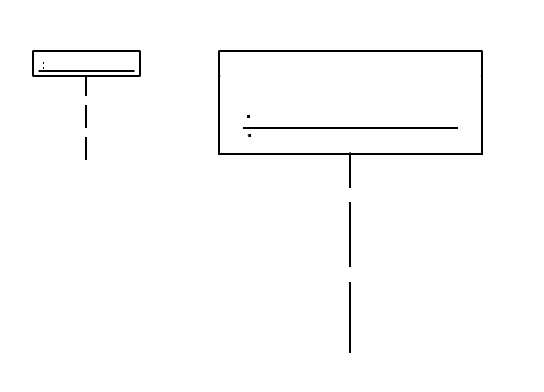
\includegraphics[width=7.35cm,height=5.295cm]{draft04-img3.jpg}
    \caption{Элемент до (слева) и после (справа) масштабирования}
    \label{scaling}
  \end{center}
\end{figure}

%{\centering 
%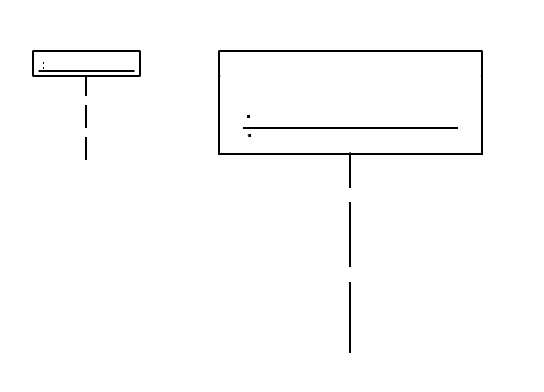
\includegraphics[width=7.35cm,height=5.295cm]{draft04-img3.jpg} \par}
%
%{\centering\selectlanguage{russian}
%Элемент до (слева) и после (справа) масштабирования
%\par}

Пользоваться такими фигурами было неудобно, а так как формат
SVG не предоставляет средства для его
расширения, была поставлена задача создания собственного языка описания
графических представлений элементов на замену SVG (и, соответственно,
реализация средств отрисовки изображений, описанных с помощью этого
языка). Основными требованиями к нему стали стала поддержка
дифференцированного масштабирования элементов – возможность при
описании элемента задавать тип масштабирования составляющих его частей.
В результате был создан язык SDF (stencil description format) и
средства его отрисовки, которые поддерживают два вида масштабирования:

\begin{itemize}
  \item Абсолютное --– размер графического примитива задается в явном виде и при
	масштабировании не меняется;\newline
    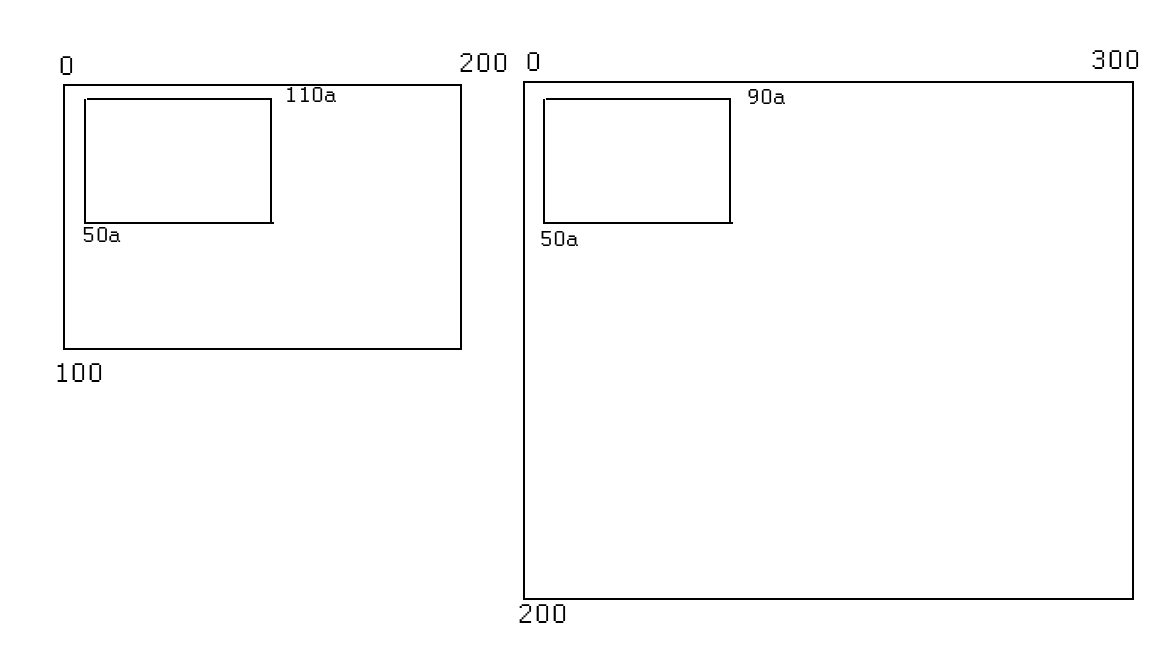
\includegraphics[width=11.622cm,height=5.646cm]{draft04-img4.jpg}
  \item Процентное --– размер графического примитива задается в процентах от
	общего размера элемента (сюда же входит и "обычное" пропорциональное
	масштабирование).\newline
    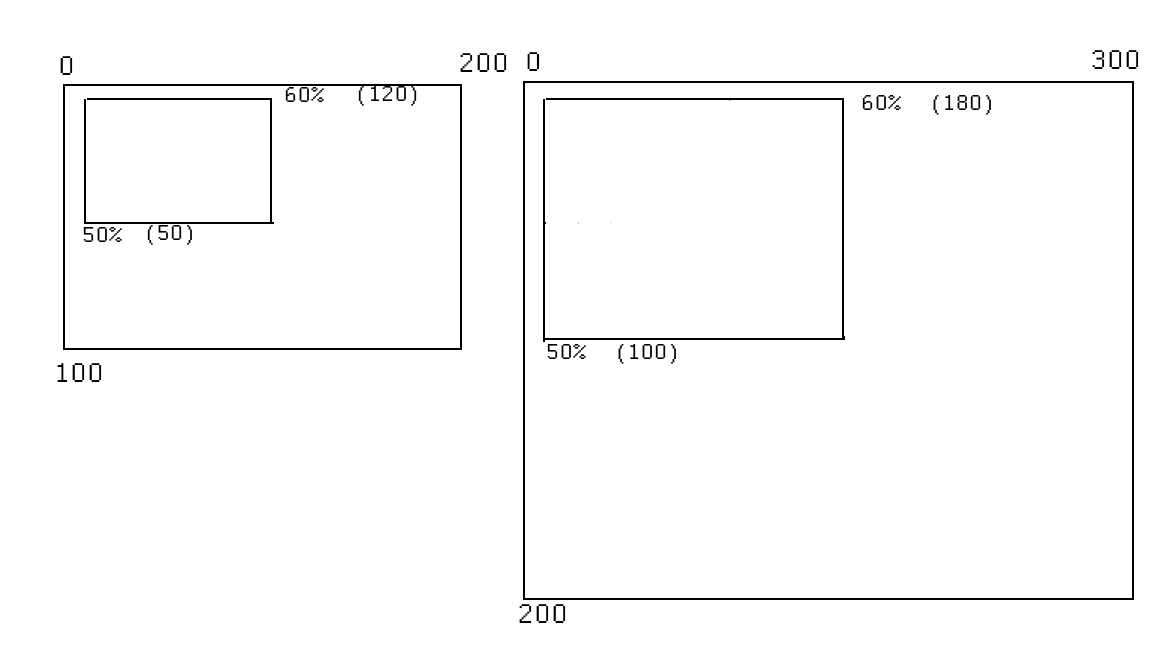
\includegraphics[width=11.582cm,height=5.927cm]{draft04-img5.jpg}
\end{itemize}

Кроме того, были созданы средства конвертации SVG-описаний в формат SDF
для преобразования большого числа уже имеющихся SVG-изображений
элементов. К тому же, мы получили гибкий формат, который можно быстро
изменять под свои дальнейшие нужды.

\section{Планы на ближайшее будущее}
\subsection{"Умная" система сборки}

Еще одним неудобством, которое испытывали разработчики CASE-пакета,
стала невозможность отслеживания изменений в XML-описаниях редакторов и
громоздкость самого цикла пересборки проекта. Дело в том, что после
изменения XML-файлов было необходимо перезапустить генератор, разложить
сгенерированные файлы в нужные места и потом уже скомпилировать
CASE-пакет. И хотя все это изначально было автоматизировано с помощью
скриптов, часто (особенно новыми членами нашей команды при попытке
"ручной сборки") некоторые этапы пропускались, что создавало
определенные проблемы и неудобства. В идеале весь этот процесс мог бы
проходить так –-- разработчик запускает утилиту make, которая собирает
генератор, запускает его на заданном наборе XML-файлов, запускает
скрипт перемещения сгенерированных файлов в нужные места (или делает
это самостоятельно), потом уже осуществляет сборку всего проекта. Таким
образом, все артефакты проекта попадают под контроль утилиты make и
изменения в них будут автоматически приводить к пересборке (или
перегенерации) нужных частей системы.

\subsection{Поддержка подключаемых модулей}

В результате проработки подобной системы сборки родилась идея о
дальнейшей модернизации архитектуры в сторону поддержки подключаемых
модулей (plug-in). Такими модулями могли бы быть редакторы или
генераторы – каждый plug-in получает некий API для взаимодействия с
графическим интерфейсом пользователя, в случае редакторов предоставляет
модели информацию об используемых элементах, предоставляет доступ к
фабрике содержащихся в них элементов и т.п. В настоящий момент эти идеи
находятся в стадии проработки.

\subsection{Метаредактор}

На определенном этапе развития проекта создание XML-описаний редакторов
уже стало казаться некоторым разработчикам неудобным и неестественным.
Была поставлена задача создания метаредактора – редактора, позволяющего
создавать метамодели редакторов визуально, генерируя по ним
соответствующие XML-описания. По сути, метаредактор предоставляет
пользователям визуальный язык, являющийся подмножеством
MOF~\cite{mof} , на котором описываются все
метамодели. Практика показывает, что достаточно реализовать лишь
небольшой набор элементов MOF: 

\begin{itemize}
  \item классы (задают множество элементов конкретного типа),
  \item ассоциации между ними (например, для задания отношения наследования),
  \item атрибуты классов (например, используемые для задания свойств элементов
	заданного типа).
\end{itemize}

На данный момент нам кажется, что этих сущностей достаточно, чтобы
описать метамодели всех возможных редакторов, поддерживаемых нашим
CASE-средством.

\section{Заключение}

Описанный в п.1-3 прототип CASE-системы был
реализован, в данный момент проводится его доработка (как в описанных
направлениях, так и в некоторых других). Параллельно с этим, группой
студентов и аспирантов кафедры системного программирования
осуществляется создание и применение генераторов для различных
предметных областей.

\pagebreak

\begin{thebibliography}{99} 

  \bibitem{real} REAL
  \bibitem{realIt} REAL-IT
  \bibitem{somethingAboutMvAndMvc} чтонить про MV/MVC
  \bibitem{bryksin} Диплом Тимофея
  \bibitem{nikandrov} Диплом Гоги
  \bibitem{simonova} Диплом Александры
  \bibitem{htmlInQt} теги HTML, поддерживаемые в Qt
  \bibitem{ice} ZeroC ICE
  \bibitem{mof} MOF
  \bibitem{svgTiny} SVG tiny
\end{thebibliography}

\end{document}
